% !TeX root = ../main.tex

\xchapter{绪论}{Introductions}

\xsection{研究背景与意义}{Research Background and Significance}

在新型飞行平台技术日渐成熟与低空应用生态加速扩张的双重推动下,低空经济作为融合空域资源开发与前沿技术应用的战略性新兴产业,正成为培育新质生产力、推动经济结构优化升级的新增长引擎。低空经济泛指在垂直高度1000米以下的空域范围内,以各类有人驾驶和无人驾驶航空器为载体,以多元化的低空飞行活动为牵引,辐射带动相关领域融合发展的综合性经济形态。它不仅有助于解决传统地面交通拥堵、提升偏远地区通达性,更是构建“空天地一体化”综合立体交通网、推动经济社会高质量发展的战略支点。作为低空经济的核心载体,以无人机(Unmanned Aerial Vehicle, UAV)和电动垂直起降航空器(electric Vertical Take-Off and Landing,eVTOL)为代表的智能航空器正发挥着前所未有的关键作用,其突出的灵活性与适应性,催生了城市空中交通(Urban Air Mobility, UAM)等新兴交通运输范式,并推动应用场景从传统的通用航空运营,广泛渗透至物流配送、农业植保、电力巡检、环境监测、应急救援乃至公共安全等众多领域,产生了颠覆性的影响。这些智能航空器正从根本上提升作业效率并重塑行业生态,凭借其低碳环保、噪声低、运行成本低等技术优势,正推动基础设施巡检、广域态势感知、应急救援等应用场景从传统人工操作向无人化智能作业模式的变革。低空经济的蓬勃发展与广泛应用,对其核心载体无人机的智能化水平提出了极高要求。然而,实现复杂动态环境下的自主感知、决策与行动,其关键在于飞行平台能否具备实时、精准、可靠的环境感知与信息处理能力。在此背景下,智能光电系统的重要性日益凸显,并已成为无人机的核心组件与实现其智能化的关键使能技术。

\begin{figure}[H]
\centering
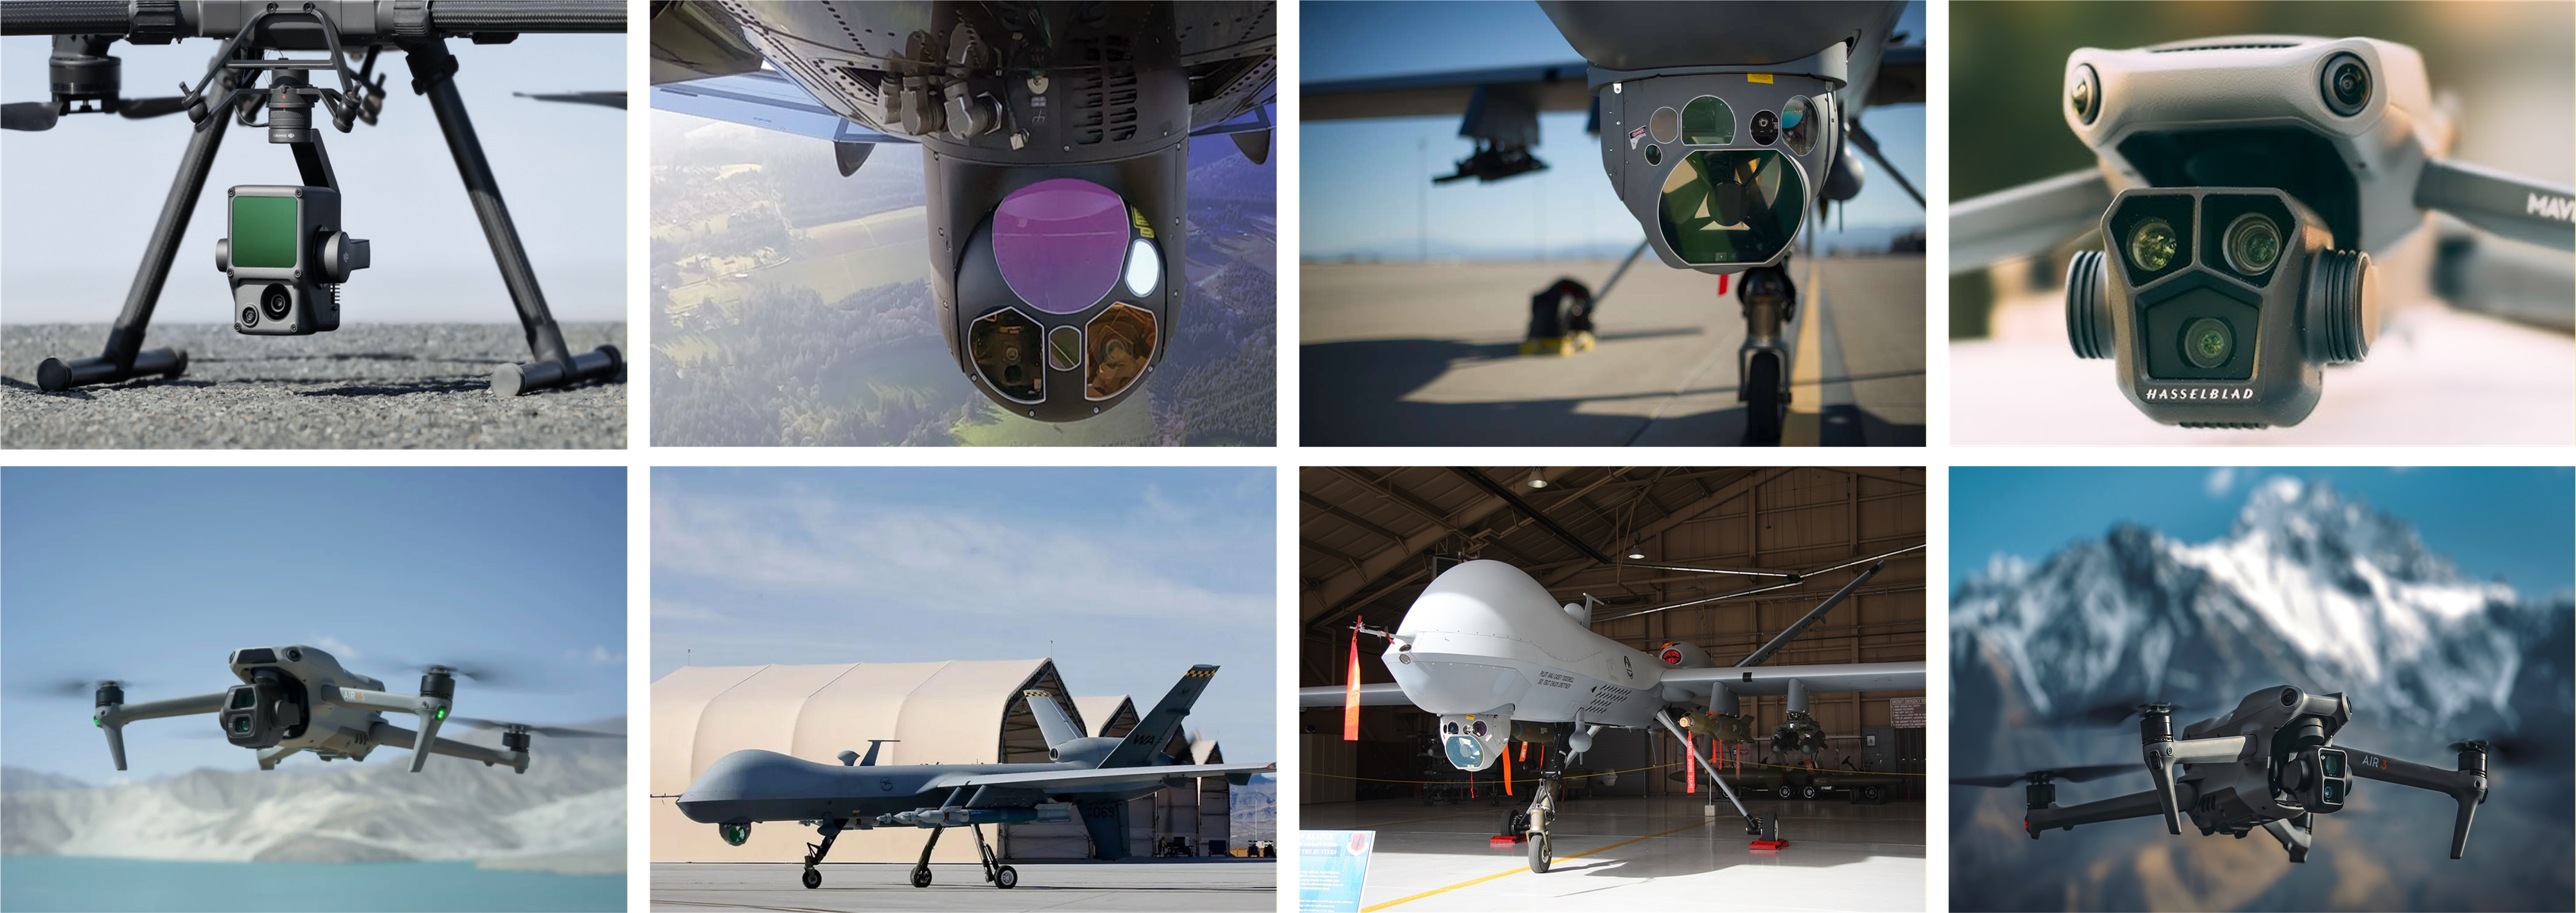
\includegraphics[width=0.98\textwidth]{uav_and_pod.png}
\caption{无人机与其搭载的光电系统}
\label{fig:uav_and_pod}
\end{figure}

无人机光电系统是一种基于光电转换原理的综合性探测系统,其核心功能是通过接收目标反射或辐射的电磁波,将其转换为电信号并进行处理,从而实现对目标的探测、识别、跟踪与测距。该系统是现代无人机实现环境感知与自主飞行的核心,其基本构成包含三大核心组件:光电传感器,稳定平台和信息处理系统。光电传感器负责捕获从紫外到远红外波段的电磁波信息。典型系统采用多谱段集成设计,主要包括:1) 可见光摄像机,基于CCD或CMOS技术,在昼间提供高分辨率图像;2) 红外热像仪,通过检测目标与背景的温差实现夜间观测,常用中波红外与长波红外波段以契合大气传输窗口;3) 激光测距仪,作为主动探测组件,通过测量激光飞行时间提供精确的目标距离信息。此外,先进系统正逐步集成短波红外、高光谱成像仪乃至激光雷达等传感器,极大丰富了信息的维度与层次。稳定平台用于隔离无人机飞行过程中产生的振动和姿态变化,确保光电传感器视轴的稳定指向。它采用多轴陀螺稳定技术,通过惯性测量单元实时感知无人机飞行带来的振动与姿态变化,并驱动伺服机构产生反向补偿运动,以维持传感器视轴的稳定指向。信息处理系统对传感器获取的原始数据进行处理、分析和利用,包括图像增强、降噪、和电子稳像等基础处理任务,运用计算机视觉与深度学习算法实现目标的自动检测、识别与持续跟踪的智能分析任务,以及对于多谱段图像、激光测距与惯性导航数据的整合压缩以及融合,生成统一的目标信息和态势数据。


无人机光电系统的发展经历了从功能单一的观测设备到多传感器融合的智能任务系统的演进。这一历程始于20世纪60-80年代,彼时的系统功能相对简单,主要以可见光电视摄像为核心,配备基础的光学望远镜和简单的机械稳定装置。系统体积重量大、分辨率和稳定性有限,且基本无法进行夜间观测。直至70年代,随着红外技术起步,系统开始集成第一代需要光机扫描的红外热像仪,采用单元或线列探测器,灵敏度较低,且整个系统的智能化程度极低,完全依赖操作员的肉眼识别和手动控制。 进入20世纪90年代至21世纪初,凝视型焦平面阵列技术和数字信号处理技术的成熟带来了性能的质的飞跃。基于锑化铟(InSb)或碲镉汞(HgCdTe)材料的焦平面阵列红外探测器成为主流,实现了高灵敏度红外成像,彩色CCD相机也取代了早期的黑白电视相机。在稳定平台方面,基于光纤陀螺或激光陀螺的多轴稳定平台成为标准配置,显著提升了稳定精度。此阶段,可见光、红外与激光测距/指示器构成的典型“三光系统”成为高端无人机的标配,并开始引入自动目标识别和电子稳像等初步智能算法,实现了从侦察到打击的一体化能力,其代表性系统如美国MQ-1B“捕食者”无人机搭载的AN/AAS-52光电系统。 从2010年至今,无人机光电系统向着多光谱、高分辨率与高度智能化方向发展。传感器范畴已远超传统可见光与红外,扩展至短波红外、中波红外、高光谱成像及偏振成像等新型传感器,例如美国Raytheon公司的RAIVEN系统融合了激光雷达以创建3D环境图像。在信息处理层面,人工智能与深度学习算法的集成,赋予了系统更强大的自动目标识别、跟踪与智能分析能力。同时,系统架构走向开放化,支持功能的快速扩展与升级。现代系统,如以色列RAFEL公司的Litening-5多功能吊舱,已演变为集情报、监视、目标捕获与侦察于一体的完整任务系统,标志着其从独立的“传感器”向“传感-互联-情报生成”综合节点的转型。

尽管无人机光电系统在技术上取得了显著进步,但就其智能化程度而言,整体仍处于初级发展阶段,尚未达到完全自主的高级智能水平。现有的智能化功能更多体现在辅助决策层面,而非完全的自主决策。在目标识别与跟踪方面,现有系统已能实现一定程度的自动检测和识别,但多局限于预设类别的目标,且对图像质量、环境条件有较高要求。目前的目标识别算法在背景简单、目标清晰的情况下表现良好,但在复杂背景或伪装欺骗条件下,性能会显著下降。具体体现在以下三个方面,首先,现有识别算法对于航拍视角下的小目标检测效果普遍不佳。 由于无人机通常在百米乃至千米级高度进行广域侦察,地面目标在图像中所占的像素占比极小,往往不足图像的0.1\%。这种小目标所携带的图像特征非常微弱,在经历了模型的下采样操作后,其细节信息几乎损失殆尽,导致主流检测模型(如YOLO、DETR等)的特征提取网络难以有效捕获其差异性特征,从而造成大量的漏检与误检。其次,现有跟踪算法在面对目标遮挡及复杂背景干扰时,难以实现稳定的持续跟踪。无人机在执行任务时,目标易被树木、建筑物等物体遮挡,或混入人群、车流等相似动态背景中。当前以相关滤波和孪生网络为代表的跟踪算法,通常不具备判丢和重捕获的能力,目标在被遮挡时模型无法及时感知,现象通常是跟踪框定在遮挡物上或跳变至其他目标,在目标重现后因模型更新错误或判别能力不足无法重新锁定正确的目标,导致跟踪失败。最后,红外图像中弱小目标识别面临着比可见光图像更为严峻的挑战。红外成像依赖于目标与背景的热辐射差异,但其固有的低分辨率、低对比度和缺乏丰富纹理细节的特性,使得小目标信噪比极低,在图像中几乎与背景噪声融为一体。这不仅使人眼观察困难,也使得通用识别算法效能骤降。如何从信噪比低、背景杂波强的红外图像中稳定、准确地分离出弱小目标,是目前智能光电处理领域一个尚未完全解决的痛点。
	
由于功耗和尺寸的限制,无人机光电系统通常采用嵌入式边缘计算设备作为信息处理核心,这类设备的计算资源、内存带宽和功耗预算都极为有限,严重制约了复杂智能算法的实时性能。目前基于Transformer的主流目标识别和跟踪算法参数量大,计算复杂度高,难以在边缘设备实现实时处理。同时,算法复杂度与精度之间的平衡面临严峻挑战,为了提升对小目标的检测能力,现有研究往往通过增加网络深度、增大图像分辨率等增加计算负载的方法,使其更加难以在边缘设备上部署,无法在边缘设备上实现端到端的实时智能感知,严重削弱了无人机在动态环境中自主感知与快速响应的能力。

综上所述,面向无人机光电系统智能化的迫切需求,以及当前光电系统在算法层面与硬件层面上面临的双重挑战,本文拟研究一套高效、高精度的多光谱智能光电处理算法,并据此设计一套与之适配的嵌入式系统架构,以提升无人机在真实复杂场景下的自主感知能力。本文将重点研究可见光航拍图像中的小目标识别,通过设计专门的特征增强模块与多尺度融合机制来提升微小目标的检测精度,探索复杂场景下的抗遮挡长时目标跟踪方法,结合重识别技术与自适应模型更新策略,确保目标在遮挡干扰下的持续稳定跟踪,同时,针对红外航拍图像中的小目标识别难题,开展面向无人机红外图像的轻量化小目标检测网络研究,结合轻量化网络探索全新的特征融合机制,提升低信噪比环境下弱小目标的检测能力,最终通过智能光电系统嵌入式架构的软硬件协同设计,构建完整的智能光电系统软硬件集成方案,实现从算法创新到系统集成的完整技术闭环,为推进无人机光电系统的智能化升级提供理论与实践支撑。



\xsection{国内外研究现状}{Domestic and International Research Status}

\xsubsection{机载光电系统总体研究进展}{Overall Research Progress of Electro-Optical Systems}

机载光电系统指的是集成在有人或无人飞行平台,用于执行侦察、监视、目标识别与跟踪等多重任务的光电系统,是一个涉及了光学、电子、机械、计算机软硬件等领域的综合系统。其工作原理是通过集成多种光电传感器,将所处环境的光学特征或红外辐射等信息转换为电信号,并经后续处理形成可供人工判读或机器自动识别的图像与数据,为侦察、跟踪、测量等任务提供关键信息输入。机载光电系统的发展经历了功能单一到高度集成化的过程,早期的光电系统只配备单一传感器,而现代光电系统则集成了多波段、多类型的传感器,并朝着与飞行平台深度耦合的方向发展。

基于多光谱探测与稳定平台技术的持续突破,目前已形成多条技术路线各异、功能侧重点不同的代表性系统。美国FLIR系统公司生产的Star SAFIRE HD光电系统是高度集成化的典范,其最多可同时装载八种传感器,包括高分辨率中波红外焦平面传感器、高清彩色可见光传感器、微光与短波红外传感器,以及激光测距仪、指示器和惯性测量组件。其可见光与红外相机均能实现120倍的光学连续变焦,视场分别覆盖29°~0.25°和40°~0.35°的范围,无缝衔接大视场搜索与小视场精细识别的任务需求。在战略侦察领域,Northrop Grumman公司为“全球鹰”高空长航时无人机设计的综合传感器套件(EISS)展现了系统级融合的先进理念。该套件集成了合成孔径雷达、移动目标指示器、高清可见光相机和第三代红外传感器,具备全天候、全时段侦察能力。其光电载荷采用全反射式双波段共孔径光学系统成像,并运用高精度两轴稳定平台与快速反射镜相结合的全数字复合控制技术,有效实现了广域扫描搜索、动目标检测、高精度稳像及像移补偿,在高速飞行条件下仍能获取稳定的高分辨率图像。

在当前技术发展背景下,前沿研究主要聚焦于系统轻量化、智能化和实时处理能力的突破。美国Logos公司开发的轻型多模式“战术光谱和侦察成像"(SPRITE)吊舱是该领域的典型代表。它将超轻型广域运动成像(WAMI)传感器、高清侦察相机和短波红外高光谱传感器集于一身,并在吊舱内集成了一个手掌大小的“多模式边缘处理器”(MMEP)。该处理器能以每秒10亿像素的极高速度处理不同类型数据,使得三种传感器能够相互指示、协同工作,极大地提升了无人机在复杂环境下发现、识别与跟踪目标的能力。高精度视轴稳定技术构成了机载光电系统成像质量保障的核心基础,其中L3Harris WESCAM公司开发的MX系列光电系统在此方面取得了显著突破。该系列产品采用创新的五轴稳定架构与独特的传感器-稳定机构隔离设计,使其集成的多种高性能传感器(涵盖1080p高清中波红外传感器、连续变焦高清可见光相机及激光测距仪等)能够获得一致的稳定性能。其采用的模块化现场可更换单元设计,使得传感器更换后无需重新校准,显著提升了系统的可维护性与适应性。以色列RAFAEL公司的RecceLite XR光电侦察系统,集成了可见光、近红外、中波红外和短波红外四种波长传感器,探测范围扩展至80公里以上,并结合先进的图像处理算法,支持广域持续监视与防区外侦察。Elbit Systems公司推出的新一代先进多传感器有效载荷系统(AMPS NG)采用了双前视红外传感器设计并增加了短波红外传感器,这种配置能有效克服高湿度、烟尘或灰尘等恶劣环境的干扰,实现了在数十公里外对地面及空中目标的高分辨率成像与稳定跟踪,展现了其在复杂环境下的适应能力。

当前机载光电系统的发展主要集中体现在硬件层面的持续优化,包括但不限于传感器谱段的扩展、探测器分辨率的提升以及稳定平台精度的改进。这些技术进步提升了系统数据采集与前端处理的性能与可靠性,但其智能化水平依然存在明显局限。具体而言,现有系统普遍缺乏对感知内容的深度理解能力,所搭载的算法多局限于基础图像增强与人工辅助识别,难以在复杂战场环境下实现真正意义上的自主探测、智能识别与决策支持。在行业应用深化与技术发展的内在驱动下,现代机载光电系统呈现出多维度的协同演进趋势。在感知层面,为适应复杂环境与多样化探测需求,系统正朝着多光谱、高分辨率与高帧频的方向发展,以全面提升环境感知精度。为实现精准观测与稳定跟踪,系统需具备更强的扰动抑制能力,并与导航定位系统深度融合,实现高精度的自主定位与目标运动分析。面对海量异构数据,信息处理系统需引入边缘计算与智能算法,实现高效的特征提取与目标识别。同时,小型化、轻量化与成本控制成为系统规模化应用的关键,这依赖于光机电一体化设计与新型材料的创新应用。最终,系统功能从单一感知向多任务集成方向发展,通过智能化处理逐步完成从数据采集设备到智能感知节点的能力升级。


\xsubsection{机载光电系统小目标检测研究现状}{Research of Small Object Detection for Electro-Optical Systems}

机载光电系统的小目标检测技术是实现远程精准感知的关键,其核心任务是在远距离成像条件下,从复杂背景中识别出像素占比极低、特征微弱的感兴趣目标。在军事侦察、灾害监测、安防巡逻等应用中,目标的远距离成像特性导致其在图像中占据极少数像素点,同时受到复杂背景杂波、低信噪比以及目标纹理信息匮乏等因素的制约。早期的研究多基于传统模型驱动方法,例如利用局部对比度测量或低秩稀疏分解理论来增强目标与背景的差异性。这类方法在简单场景下具有一定效果,但其性能高度依赖于人工设计的先验假设,在面临强背景干扰、目标尺度变化或低照度条件时,常出现虚警率升高、鲁棒性不足的问题。随着人工智能技术的发展,基于深度学习的方法已成为当前研究的主流。深度神经网络通过端到端的学习方式,能够自动从大规模数据中提取更具判别力的特征,显著提升了模型在复杂环境下的泛化能力。为应对上述挑战,现有小目标检测方法通常在通用目标检测的成熟框架中引入针对性设计,通过改进网络结构、优化特征提取机制和增强上下文建模能力等方式,解决小目标检测中的难题。具体的方法包括:数据增强,多尺度融合,超分辨率,上下文建模,注意力机制,聚焦检测。

\subsubsection{基于图像增强的小目标检测方法}

在深度学习领域,训练样本的不足会直接导致模型性能的显著下降。因此,利用大量数据进行训练是确保模型获得强大泛化能力的关键。数据增强技术是丰富数据集多样性、提升模型鲁棒性与泛化能力的常用策略,同时也有助于缓解因数据集中不同尺度目标分布不均衡而导致的检测精度下降问题。早期的数据增强主要依赖于基础的几何变换(如旋转、缩放、裁剪和平移)和颜色变换来增加数据多样性,同时还有经典的Mosaic\cite{YOLOv4}、MixUp\cite{Zhangmixup}和CutMix\cite{yun2019cutmix},但这些通用方法对中大型目标的性能提升通常优于小目标,在小目标检测场景下效果有限。因此,越来越多的学者开始专注于研究针对小目标检测的专用数据增强技术。Kisantal等人\cite{kisantal2019augmentation}提出了两种创新策略:一是对包含小目标的图像进行过采样,二是对小目标进行多次复制-粘贴。他们通过系统实验比较了不同复制策略,发现复制全部小目标的效果最优,而仅复制单个小目标虽然能提升小尺度目标检测,但会对大尺度目标产生负面影响。为进一步优化上述方法,Chen等人\cite{ChenRRNet}提出了自适应数据增强技术,通过引入反馈机制解决随机复制粘贴可能导致的背景失配与目标尺寸失配问题。Xiao等人\cite{xiao2023tiny}则提出了Copy-Reduce-Paste方法,该方法通过复制并调整微小目标的大小和位置,再粘贴到图像的不同区域,增加了微小目标在训练数据中的比重,从而在损失函数中给予微小目标更多的权重,改善了训练样本的平衡性。


在数据处理层面,Ünel等人\cite{ozge2019power}提出了一种创新的分块方法,通过裁剪图像增大小目标的相对面积,同时保留完整图像输入以确保对大目标的检测能力,最终通过融合多尺度检测结果实现性能提升。针对预训练与微调阶段的数据尺度不匹配问题,Yu等人\cite{YuScaleMatch}提出了尺度匹配策略,通过裁剪减小尺度差距,这一方法提升了FPN检测器5\%的检测性能。Lin等人\cite{lin2019san}提出一种新的尺度感知模块(scale-aware network,SAN)通过自适应重采样策略解决了遥感影像中的尺度不连续性问题,Zoph等人\cite{zoph2020learning}提出的自搜索学习框架采用强化学习方法自动探索最优数据增强策略组合,为小目标检测的性能优化开辟了新途径。

尽管数据增强方法通过增加小目标数量来缓解正样本稀缺这一核心问题,但其自身存在明显的局限性。这类方法通常表现出性能提升的不稳定与较差的迁移性,即某种增强策略在特定数据集或模型上有效,但难以泛化至其他场景。其根本原因在于,许多数据增强方法(如简单的复制-粘贴)可能引入不真实的上下文或背景失配问题,未能从根本上优化模型对于小目标特征的学习能力。


\subsubsection{基于多尺度融合的小目标检测方法}
在基于深度学习的目标检测中,小目标的弱特征表示是导致其检测性能不佳的主要原因。经过卷积和池化的多次下采样操作后,最终特征图中包含的小目标特征信息极少。此外,神经网络会生成不同分辨率的特征图,深层特征图具有更大的感受野、更强的语义信息,但其分辨率较低,丢失了大量细节信息。相反,浅层特征图分辨率较高,保留了丰富的细节和位置信息,但缺乏足够的语义信息。为了同时利用深层特征的丰富语义和浅层特征的空间细节,研究者们主要沿着两条技术路径进行探索:一是构建专用尺度检测器,通过多分支架构或定制化训练方案使不同层级负责不同尺度的目标;二是进行分层特征融合,整合不同深度的特征以构建对小目标更强大的表征能力。这两种路径的核心都在于最大限度地减少特征提取过程中的信息损失。

\paragraph{专用尺度检测器}
该类方法的本质是令网络中不同深度的特征图专注于检测相应尺度的目标,从而实现更优的感受野匹配。早期工作如Yang等人\cite{Yang2016Exploit}提出的尺度依赖池化(scale-dependent pooling,SDP),通过为小目标选择合适的特征层进行后续操作。MS-CNN\cite{Cai2016MultiScale}在不同中间层生成候选区域,使每一层专注于特定尺度范围的目标。单阶段检测器如 YOLO系列\cite{redmon2018yolov3},通过添加并行分支,利用高分辨率特征负责小目标检测。具有里程碑意义的工作是 Lin 等人\cite{FPN}提出的特征金字塔网络 (Feature Pyramid Networks, FPN)。FPN通过自上而下的路径和横向连接,构建了具有强语义信息的多尺度特征金字塔,并依据目标尺寸将其分配至不同金字塔层级进行检测。这种简单高效的设计已成为现代检测器的标准组件,并催生了一系列变体,如NAS-FPN\cite{NAS-FPN}和 Recursive-FPN\cite{DetectoRS}。此外,研究者还尝试组合多个尺度专用检测器,Li等人\cite{Li2018ScaleAware}构建了并行子网络,其中小尺度子网络专门用于检测小尺寸行人。TridentNet\cite{li2019scale}构建了具有不同膨胀卷积的并行多分支架构,使每个分支对特定尺度目标具有最优感受野。QueryDet\cite{Yang2022QueryDet}设计了级联查询策略,有效避免了在低层特征上的冗余计算,使得网络能够高效地利用高分辨率特征图检测小目标。在训练策略上,研究者们也提出了针对性的数据准备方法。Singh等人\cite{Singh2017SNIP}提出了尺度归一化图像金字塔,该模型只对落在预定尺度范围内的目标实例进行训练,其余则被忽略,从而确保小目标能在最合理的尺度上被处理而不影响中大目标的性能。后续的 Sniper\cite{sniper2018}从多尺度图像金字塔中采样以进行高效训练。Najibi等人\cite{najibi2019autofocus}提出了一种由粗到细的检测流程,仅处理在较细尺度上可能包含小目标的区域。Chen等人\cite{chen2021scaletraining}则设计了一种反馈驱动的训练模式,动态指导数据准备并平衡小目标的训练损失。


\paragraph{分层特征融合}
深度神经网络生成具有不同空间分辨率的层次化特征图,低层特征蕴含丰富的细节和定位信息,而高层特征捕获更强的语义信息。对于小目标检测任务,深层特征可能因小目标特征消失而失效,而浅层特征又易受光照、形变等因素干扰,分类辨识度低。为克服此困境,特征融合方法通过整合不同深度特征,以获得对小目标更鲁棒的表征。受FPN启发,PANet\cite{Liu2018PANet}通过增加自底向上的路径增强,利用精准的定位信号丰富了深层特征。Tan等人\cite{TanEfficientDet}提出了双向特征金字塔网络,以更高效、直观的方式进行多尺度特征融合,旨在为小目标提供更合适的表征,并实现更好的精度效率平衡。Zhang等人\cite{ZhangMFR-CNN}将多个深度上的RoI池化特征与全局特征拼接,为小目标获得更具判别力的表示。Woo等人\cite{Woo2017StairNetTS}提出的StairNet利用反卷积放大特征图,这种基于学习的上采样函数能产生更精细的特征,并促进不同金字塔层级间信息的有效传播。M2Det\cite{M2Det2019aaai}构建并行分支以级联方式描述从浅到深的特征,并利用U形模块捕获小目标的更多细节。Liu等人\cite{Liu2020IPGNet}提出的IPG-Net,将图像金字塔得到的不同分辨率图像输入特定变换模块,以补充空间信息和细节。Gong等人\cite{Gong2021EffectiveFPN}设计了一种基于统计的融合因子,用以控制相邻层级间的信息流。针对FPN类方法中存在的梯度不一致问题,SSPNet\cite{Hong2022SSPNet}通过强调不同层级的特定尺度特征,并利用FPN中相邻层级的关系来实现更合理的特征共享。


专用尺度检测器致力于在最合理的尺度上处理小目标,而基于融合的方法旨在弥补低金字塔层级与高层级之间的空间和语义差异。然而,前者通常直接将不同尺寸目标映射到对应层级,这可能因单层信息不足而误导检测器,后者则面临网络内信息流并不总是对小目标表征有利的问题。研究者的目标是既要赋予低层特征更多语义,又要防止小目标的原始响应被深层信号所淹没。如何在增强语义与保留细节之间取得最佳平衡,仍是当前多尺度融合技术面临的核心困境。

\subsubsection{基于超分辨率的小目标检测方法}
小目标检测的本质困境在于其有限的像素数量所导致的特征信息匮乏,尽管多尺度融合等方法试图从空间维度上弥补信息损失,但直接从图像层面提升小目标的分辨率与质量是另一条更直接的解决思路。超分辨率技术旨在从低分辨率图像中恢复出对应的高分辨率图像。高分辨率图像能够提供更多原始场景的细节,这为小目标检测提供了有力的支撑。近年来,基于生成对抗网络(GAN)\cite{Goodfellow2014GAN}的算法在图像超分领域取得了显著进展,并被成功应用于小目标检测任务中。典型的基于GAN的超分辨率框架包含两个核心子网络:一个生成器网络和一个判别器网络。生成器负责以低分辨率的小目标特征或图像块作为输入,生成高分辨率输出,试图“欺骗”判别器。判别器则作为一个对手,努力区分输入是来自真实的高分辨率图像,还是生成器产生的“伪造”超分图像。通过这种对抗性训练,生成器被驱动学习从低分辨率小目标到高分辨率表示的复杂映射,从而恢复出对小目标分类与定位至关重要的细节信息。

Perceptual GAN\cite{Li2017PerceptualGA}是首次将GAN应用于小目标检测任务的代表性工作。该模型引入了一个新颖的条件生成器,它以小目标的低层特征作为输入,生成具有更多细节的超分特征表示。生成器内部包含多个残差块,用于学习小目标与相似大目标之间的特征差异。判别器包含两个分支:对抗分支负责区分生成的小目标超分区域与真实的大目标区域,感知分支则直接在生成的超分表示上执行常规的目标检测任务。在训练中,两个分支都致力于最小化各自的损失,生成器被训练成尽可能使判别器做出错误判断,从而形成有效的对抗学习。SOD-MTGAN\cite{Bai2018SODMTGAN}为了解决生成图像不够清晰的问题,在标准GAN框架中引入了细化模块。判别器被设计为一个多任务判别器网络,同时执行三个任务:区分图像的真伪、预测目标类别以及优化边界框回归。分类损失和回归损失会反向传播到生成器,从而直接指导生成器产生更易于被准确分类和定位的超分图像。生成器的总损失函数由对抗损失、像素级均方误差损失、分类损失和边界框回归损失共同构成,这种多目标优化强制要求重建的图像不仅在视觉上逼真,而且必须包含对检测任务有益的高频细节。JCS-Net\cite{Pang2019JCSNet}专注于小尺度行人检测,它将分类子网络和超分辨率子网络集成在一个统一的架构中。超分辨率子网络采用了类似于VDSR\cite{Kim2016VDSR}的残差架构,通过探索大尺度行人与小尺度行人之间的关系,来恢复小尺度行人的细节信息。因此,重建后的小尺度行人特征既包含了原始信息,也融入了超分子网络输出的增强信息。在训练阶段,该模型通过结合分类损失和超分辨率损失进行端到端优化,并使用多层通道特征\cite{Cao2017MCF}与多尺度表示来进一步增强检测性能。

使用超分辨率的方法能够有效增强图像的细节信息,但是GAN本身训练难度大,生成器与判别器之间的动态平衡不易达成,训练过程的不稳定会直接影响最终模型的性能,在训练过程中,如果生成器只能产生有限多样性的样本,学习过程可能会过早停滞,导致生成质量下降,进而增加最终检测的误差。

\subsubsection{基于上下文建模的小目标检测方法}
小目标由于自身像素有限、特征表达能力弱,仅凭其自身信息难以实现精准的识别与定位。在此背景下,利用其周围的上下文信息成为提升小目标检测性能的关键途径之一。上下文信息提供了目标所处环境或其与周围元素的关联性线索,能够为判别小目标提供辅助依据。根据信息提取范围的不同,上下文建模可分为全局语义建模和局部上下文建模,全局语义建模关注整幅图像的统计特性与场景语义,为理解目标出现的宏观环境提供指导,局部上下文建模聚焦于目标邻近区域的细节特征,通过利用目标与周边像素、纹理或相邻物体之间的空间与语义关系,来补偿小目标自身的信息缺失,从而增强其表征的区分度与鲁棒性。

局部上下文主要指目标紧邻区域的像素级信息,如边缘、颜色和纹理等。一种直接且有效的利用方式是通过扩大检测窗口来包含更多的周围环境。Cai等人\cite{Cai2016MultiScale}提出将目标的边界框扩大至原区域的1.5倍,以此引入更丰富的周边信息。这些额外的上下文信息随后与目标自身的特征相结合,共同输入检测层进行预测。Fu等人\cite{fu2017dssddeconv}通过采用带有“跳跃连接”的反卷积层来增强特征的语义信息。与简单地在卷积层上堆叠反卷积层不同,该方法设计的反卷积层更浅,并使用了逐元素乘积操作进行特征融合,从而在小目标检测上取得了更好的效果。CAB-Net\cite{Cui2022ContextAwareBN}通过设计独特的上下文感知模块,采用金字塔扩张卷积有效融合了多层级上下文信息,同时保持了特征图的原始分辨率,显著提升了小目标检测精度。SEPN\cite{Sun2022SEPNet}构建了专门的上下文增强模块来提取多尺度特征,该模块核心由并行双分支构成:ASPP分支用于扩大感受野以捕捉更广泛的上下文信息,而金字塔卷积分支补充了ASPP卷积过程中可能丢失的细节特征,二者协同工作共同增强了模型对小目标的表征能力。Corsel\cite{Corsel2023TemporalContext}等人提出了一种基于YOLOv5的时空算法,通过利用视频序列中可用的时序上下文信息,在人员检测和空中监控领域内提高小尺寸运动物体的识别率。Zhang等人\cite{Zhang2018RefineDet}采用了自上而下的路径,将高层特征图的丰富语义信息传递并融合到细节更丰富的低层特征中。这种信息流动方式有效地增强了用于检测小目标的低层特征的语义表示能力。

尽管上下文信息能有效补偿小目标自身特征的不足,但其引入并非总是有益的。冗余或不相关的上下文信息会引入显著的噪声,干扰模型对目标本身的判断,甚至导致性能下降。


% Zagoruyko等人\cite{zagoruyko2016multipath}则采用了多尺度策略,生成了四种尺度(1x, 1.5x, 2x, 4x)的区域提议框。这些不同尺度的区域经过ROI池化后,将其特征拼接起来,再送入后续的分类与检测网络,使得模型能够从多种感受野中捕捉对识别小目标有益的局部线索。语义上下文侧重于利用场景中更高层次的、具有明确语义的信息来辅助推断目标的位置或类别。

\subsubsection{基于注意力机制的小目标检测方法}
人类视觉系统能够快速聚焦于场景中的关键部分并忽略无关信息,这种高效的认知机制被称为视觉注意力机制。受此启发,注意力机制在计算机视觉领域得到了广泛研究与应用。其核心在于通过为特征图的不同部分分配差异化权重,从而突出有价值的信息区域,同时抑制无关或冗余的部分。在小目标检测任务中,目标像素稀少,其特征极易被复杂的背景和噪声所淹没。因此,可以利用注意力机制这一优势,引导模型聚焦于那些可能包含小目标的微小区域,从而在特征层面最大限度地减少背景污染,增强小目标的特征响应。此方法设计灵活,即插即用,能够被嵌入到几乎所有主流的目标检测架构中,因此被广泛使用。

研究者们提出了多种创新的注意力模型来应对小目标检测的挑战,受人类认知过程启发的KB-RANN模型\cite{yi2019kbrcann},将长短期注意力神经网络引入检测框架,通过模拟人类视觉系统的持续性关注机制,使模型能够聚焦于图像中的关键区域。在此基础上,SCRDet\cite{Yang2019SCRDet}提出了一个创新性的旋转目标检测架构,其中集成了经过监督训练的像素注意力和通道注意力模块,实现了从小目标区域中有效分离噪声。随着anchor-free检测范式的兴起,FBR-Net\cite{Fu2021AnchorFree}通过引入层级注意力机制,在FCOS\cite{Tian2022FCOS}检测器的基础上实现了特征金字塔各层级间的自适应特征均衡,显著提升了复杂场景下的小目标检测能力。与此同时,研究者们从不同角度完善了注意力机制的应用:Lu等人\cite{Lu2021AttentionFFSSD}设计的双路径模块通过并行处理实现了关键特征的增强与非目标信息的抑制,MSCCA\cite{Ran2021Lightweight}通过用增强通道注意力块替代传统卷积组件,构建了参数效率更高的轻量级检测器,而Li等人\cite{Li2021CrossLayerAN}提出的跨层注意力模块则通过加强不同层级特征间的交互,获得了对小目标更强的特征响应。这些方法虽采用不同的技术路径,但其核心都是通过注意力权重的重新分配来增强小目标特征表示的有效性。

尽管注意力机制为小目标检测带来了性能提升,但其应用仍面临两大挑战。首先,性能的提升往往以高昂的计算开销为代价。注意力机制中的相关运算(如大规模矩阵乘法)会大幅增加模型的计算复杂度和推理时间。其次,当前大多数注意力范式缺乏明确的、直接的监督信号,其参数优化过程依赖于最终检测任务的损失回传,有可能限制了注意力模块学习到最精准的聚焦区域。


\subsubsection{基于聚焦检测的小目标检测方法}
在高分辨率图像中,小目标的分布呈现非均匀性,传统的分块检测策略会导致大量计算资源浪费在无目标的空背景区域。为了解决这一问题,研究者提出聚焦检测的方法:通过先定位潜在目标区域再进行精细检测的两阶段流程,提升了检测精度。这类方法的核心思想是打破传统处理高分辨率图像的固定流程,首先提取出可能包含目标的候选区域,随后在这些区域上执行后续检测任务。这种机制确保了小目标能够在更高分辨率下被处理,从而缓解了因下采样导致的信息丢失问题,提升了小目标的特征表示质量。

代表性工作ClusDet\cite{Yang2019ClusteredOD}通过充分挖掘目标间的语义和空间信息生成聚类区域,进而实施检测。随后的研究沿袭了这一思路并从不同角度进行深化:Duan等人\cite{Duan2021CoarseGrainedDM}与Li等人\cite{Li2020DMGOD}分别利用像素级监督进行密度估计,生成能精确表征目标分布的密度图,CRENet\cite{Wang2020ClusteringADR} 设计了自适应聚类算法来搜索目标聚集区域。另一方面,针对固定尺寸输入导致的漏检问题,有研究采用实时切片方法检测高分辨率航拍图像中的行人与车辆。与之理念相似,Deng等人\cite{Deng2021GLSAN}和Xu等人\cite{Xu2021AdaZoom}分别通过设计超分辨率网络和强化学习框架,实现了对局部区域的分辨率提升和自适应缩放聚焦。Leng等人\cite{Leng2023ParetoRefocusing}在传统区域挖掘基础上引入了区域特异性上下文学习模块,有效增强了对挑战性区域内小目标的感知能力。F\&D框架\cite{Koyun2022FocusAndDetect}通过聚焦网络检测候选区域并将其裁剪缩放到更高分辨率,为实现小目标的精准检测提供了解决方案。

与传统的滑动窗口相比,聚焦检测方法通过自适应裁剪和灵活缩放操作实现了计算资源的优化配置,小目标可在更高分辨率下处理以保留细节,而大目标则在相对较低分辨率下检测,这显著减少了推理过程中的内存占用并降低了背景干扰。然而,该类方法必须解决“聚焦何处”这一关键问题,现有方案主要依赖于辅助架构(如分割网络和高斯混合模型),使端到端优化过程复杂化。


\xsubsection{机载光电系统目标跟踪研究现状}{Research of Single Object Tracking for Electro-Optical Systems}
单目标跟踪是机载光电系统实现持续监视、精确定位与智能决策的核心,在军事侦察、安防巡逻等任务中具有不可替代的关键作用。该功能的目标是在视频序列中持续定位特定目标,其工作模式是在首帧获取目标初始位置信息后,在后续帧中实现自主定位与持续跟踪。单目标跟踪算法的发展历程经历了从基于相关滤波的传统判别式方法,到基于孪生网络的模板匹配方法。近年来,Transformer架构的引入推动了跟踪技术的发展,自注意力机制能够有效建模复杂时空依赖关系,提升算法对复杂背景下目标形变及快速运动等挑战的适应能力。下面将分别介绍判别式模型的方法,基于孪生网络的方法和基于Transformer的方法。

\subsubsection{基于判别式模型的单目标跟踪方法}
判别式跟踪器将单目标跟踪问题定义为一个二分类任务,其核心是训练一个外观模型,通过最小化判别性损失函数,来区分包含目标的正面样本与来自背景区域的负面样本。此类方法的一个关键特性在于其在线学习和模板更新机制,这使得跟踪器能够在跟踪过程中实时适应目标的外观变化、及环境改变。早期的判别式跟踪器主要依赖于手工特征(如HOG\cite{Dalal2005HOG})和简单分类器(如支持向量机或岭回归),后续研究则转向使用深度特征和基于优化的预测模型。其中,基于相关滤波的跟踪器在判别式跟踪器发展中发挥了关键作用。

相关滤波类方法的核心是在线学习一个线性滤波器,通过求解一个岭回归问题,使得该滤波器能够从目标周围的背景区域中有效区分出目标图像块。其最主要的创新在于利用快速傅里叶变换将计算转换到频域,并利用循环互相关的性质,实现了快速的滤波器训练和更新。在跟踪过程中,相关滤波器被应用于一个以目标上一帧位置为中心的搜索窗口上,滤波器输出的最大响应值位置即被判定为目标的当前位置。在每一帧处理完毕后,跟踪器会在线更新滤波器权重,使模型能够动态适应目标外观变化,部分方法还可通过选择最高相关输出对应的尺度实现目标尺度估计。MOSSE\cite{Bolme2010MOSSE}是早期相关滤波跟踪器的代表之一。它提出了一种简单且实时的跟踪方法,对尺度、光照、姿态和非刚性形变具有鲁棒性。相较于之前需要大量训练样本的相关滤波方法,MOSSE仅使用单帧图像训练滤波器,降低了数据需求。KCF\cite{Henriques2015KCF} 在MOSSE的基础上引入了核化技巧与多通道特征(如HOG)支持,进一步提升了判别能力和特征表示。KCF充分利用了图像块平移后的循环结构,通过应用离散傅里叶变换,降低了存储和计算复杂度,即使使用更丰富的特征表示也能实现实时处理。SRDCF\cite{Danelljan2015SRDCF}针对常规互相关滤波跟踪器因循环卷积而产生的边界问题,引入了空间正则化项,根据滤波器系数的空间位置对其进行惩罚。这使得模型能够从包含更丰富负样本的更大图像区域中学习,同时将注意力集中于目标本身。该方法通过在频域中利用正则项的稀疏性,并采用高斯-塞德尔求解器进行在线优化,保持了计算效率。

随着深度学习的兴起,相关滤波开始与神经网络架构融合。CFNet\cite{Valmadre2017CFNet}将在线相关滤波器作为一个可微分层集成到一个浅层孪生网络中,实现了跟踪模型与特征表示的端到端学习,其关键创新在于将相关滤波器视为一个封闭的优化模块,并通过反向传播将其嵌入网络。后续的高级判别式跟踪框架不再以相关滤波为核心,DiMP\cite{Bhat2019DiMP}通过改进目标模型的学习过程,增强了跟踪器从背景干扰中区分目标的能力。它将目标模型学习视为一个判别性损失函数优化问题,并利用元学习优化器在线更新模型。此外,DiMP集成了一个并行的IoU预测分支用于精确的边界框估计。PrDiMP\cite{Danelljan2020PrDiMP}在DiMP的基础上,通过将目标中心定位和边界框回归重新设计为概率回归任务,进一步提升了跟踪器的鲁棒性。它直接通过网络架构对目标状态的条件概率密度进行建模,而不假设预定义的分布,使跟踪器能够表示标注本身及目标状态的不确定性。


\subsubsection{基于孪生网络的单目标跟踪方法}
孪生网络跟踪器是单目标跟踪领域的一个重要范式,其核心思想是将跟踪任务定义为目标模板与搜索区域之间的相似性匹配问题。典型的孪生网络由两个权值共享的分支构成:模板分支处理第一帧中的目标图像块,搜索分支处理当前帧中的候选区域。这两个分支通过一个共享的主干网络将输入映射到一个公共的特征空间,随后通过计算两者之间的相似度来定位目标。此类方法通常在大规模数据集上进行离线训练,以学习一个通用的匹配函数,从而在在线推理时无需复杂的模型更新即可实现目标跟踪。孪生网络跟踪器通过引入新的回归头、更新机制、更深的主干网络以及注意力模块等创新,在鲁棒性和准确性上不断进步。

SiamFC\cite{Bertinetto2016SiamFC}开创性地将用于相似性学习的全卷积孪生网络引入跟踪领域。该网络通过两个相同的分支提取模板和搜索区域的特征,再经过一个互相关层,生成一个密集的响应图来指示目标的位置。这种架构无需在线更新模型,并通过使用图像金字塔来应对尺度变化。SA-Siam\cite{He2018SASiamese}提出了一个双重的孪生网络结构,通过融合互补的表观特征和语义特征来提升模型的泛化能力。该网络包含两个独立训练的分支:表观分支保持SiamFC的结构进行相似性学习,语义分支从一个预训练的分类网络中提取高层语义特征。两个分支仅在推理时进行融合,并引入通道注意力机制来增强语义分支中的目标特异性表示,从而提升了对外观变化的鲁棒性。SiamRPN\cite{Li2018SiamRPN}将区域提议网络 引入孪生框架,是推动该领域发展的关键一步。RPN的加入使得网络能够同时进行前景背景分类和边界框回归,从而实现了更精确的尺度与长宽比估计,摒弃了SiamFC中使用的多尺度搜索策略。该模型将跟踪建模为一个局部一次性检测任务,其中模板分支充当元学习器,为搜索分支生成检测核。DaSiamRPN\cite{Zhu2018DaDASiamRPN}针对训练数据中语义背景与非语义背景不均衡的问题,提出了干扰物感知的训练策略。在离线训练中,它通过引入来自同类和不同类别的语义负样本对,使网络学习更具判别力的表征。在推理时,它采用由局部到全局的搜索策略,并结合困难负样本挖掘,有效增强了跟踪器的短期精度。SiamRPN++\cite{Li2019SiamRPN++}解决了早期孪生网络无法使用ResNet\cite{He2016ResNet}等深层主干网络的限制,实现了更深网络的端到端训练。此外,该方法通过多层特征聚合以及轻量的深度互相关模块,在提升精度的同时减少了参数量,稳定了训练过程。

SiamFC++\cite{Xu2020SiamFC++}通过解耦分类与回归分支,将粗略的目标定位与精确的边界框预测分离。该模型采用无锚框的逐像素预测策略,避免了对目标先验尺度的依赖,并引入一个质量评估分支来估计边界框预测的可靠性,以解决高分类置信度与差定位结果不匹配的问题。SiamAttn\cite{Yu2020SiamAttn}针对固定模板在应对目标外观变化时的局限性,在孪生架构中引入了可变形孪生注意力模块。该模块结合了可变形自注意力和交叉注意力,分别用于建模帧内上下文以及模板与搜索区域之间的相互依赖关系,从而实现了对目标模板的自适应更新,提升了在背景杂乱情况下的鲁棒性。SiamDMU\cite{Liu2024SiamDMU}提出了一个双掩码模板更新方法。该方法在SiamRPN++的框架上,增加了一个由掩码增强块和模板更新块构成的模板更新模块。该模块利用语义分割和长期运动信息,在图像级别而非特征级别更新模板,保留了高分辨率的空间细节,从而在严重外观变化下实现鲁棒跟踪。Siam R-CNN\cite{Voigtlaender2020SiamRCNN}为长期跟踪设计了一个两阶段的孪生重检测框架。它抛弃了围绕先前预测进行局部搜索的策略,转而执行全图范围的全局重检测。其核心是轨迹动态规划算法,该算法综合考虑来自第一帧模板和前一帧的重检测结果,形成时空轨迹,从而实现鲁棒的目标关联与干扰物抑制。


\subsubsection{基于Transformer的单目标跟踪方法}
% Transformer架构因其在自然语言处理任务中的成功而被引入计算机视觉领域,并在语义分割、目标检测、图像分类等任务中展现出卓越性能。与主要关注空间信息的孪生网络跟踪器以及结合历史预测进行模型更新的在线方法不同,Transformer通过注意力机制同时建模帧内与帧间的依赖关系, 与依赖局部感受野的卷积神经网络不同,Transformer采用全局注意力能更好地捕获长距离上下文信息。基于Transformer的跟踪方法利用编码器-解码器架构、自注意力等关键组件来增强特征表示和目标定位能力。根据架构设计,现有Transformer跟踪器可分为两大类:混合Transformer跟踪器和完全Transformer跟踪器。
% 混合Transformer跟踪器将Transformer模块嵌入到已有的孪生或判别式跟踪框架中,以增强其性能,解决CNN架构中感受野有限、全局上下文建模不足等问题。TransT 是早期将注意力架构引入跟踪的代表性工作。它完全取代了孪生框架中传统的基于互相关的特征融合方式,设计了一个由基于多头自注意力的ECA模块和基于多头交叉注意力的CFA模块构成的融合网络。这种设计能更好地捕获全局上下文,在整合模板与搜索区域特征时保留语义信息,从而在外观变化和相似物体干扰下实现鲁棒跟踪。TrDiMP与TrSiam 通过为判别式和孪生跟踪器引入Transformer架构来建模视频帧间的时序依赖。它们设计了一个并行的编码器解码器框架,编码器用于增强多帧间的模板特征,解码器则将历史模板的空间掩码和特征传播到当前搜索区域,共享注意力权重和轻量级设计保证了计算效率。ToMP 针对像DiMP这类基于优化的判别式跟踪器的局限性,使用基于Transformer的模型预测器取代了传统的模型优化器。该设计能够对训练帧和测试帧进行全局上下文建模,实现转导式的目标模型预测,并通过联合预测分类和回归权重,实现了更鲁棒的定位和目标估计。
% 完全Transformer跟踪器不依赖原有的孪生或判别式跟踪框架,从头构建基于Transformer的独立架构。为了克服卷积网络难以捕捉长距离依赖关系的问题,STARK 引入了具有编码器解码器架构的模型。其编码器通过联合处理初始模板、动态更新模板和当前搜索区域的特征,捕获全局上下文关系,利用多头自注意力强化时空编码。一个轻量级解码器学习单个查询向量来预测目标位置,并提出了一个基于角点的全卷积预测头,简化了跟踪流程。CSWinTT 引入了多尺度循环移位窗口注意力机制,将注意力计算从像素级提升到窗口级,以保持物体结构并实现更局部化的匹配。其循环移位策略结合空间正则化注意力掩码,在生成多样窗口样本的同时抑制了边界效应。MixFormer 提出了一种紧凑的端到端架构,其核心是混合注意力模块,该模块能够同时执行自注意力和交叉注意力操作,统一了特征提取和信息集成阶段。它采用CvT作为主干网络,并引入非对称注意力方案以提升效率。SwinTrack 是一个基于Swin Transformer的单目标跟踪框架。它将模板和搜索区域特征拼接后通过共享主干进行联合建模,并引入一个运动令牌来捕获目标的历史轨迹,从而在解码器中增强时序感知能力。

% 两阶段跟踪器分别从模板区域和搜索区域独立提取特征,并在后期进行特征融合以建立关联模型,其对目标的感知能力较弱,目标与背景的区分度有限。为解决这一问题,OSTrack提出了一种单流、单阶段的Transformer 框架,该框架在初始阶段实现模板与搜索区域之间的双向信息流动,将特征提取与关系建模统一起来。该方法通过直接拼接两个输入,利用自注意力机制学习具有目标感知能力的特征,无需再设计独立的交叉注意力模块。SeqTrack引入了新颖的Seq2Sqe学习框架,将目标跟踪视为自回归序列生成任务。该方法将边界框坐标离散化为令牌序列,并使用普通编码器解码器Transformer学习生成它们,编码器联合提取模板和搜索图像的特征,而因果解码器自回归地预测边界框。
% 传统的单目标跟踪方法依赖于针对特定模态的设计,这些方法采用定制化架构,参数量冗余且性能有限。OneTracker [42] 通过引入一种统一高效的双模态(RGB与RGB+X)跟踪框架来上述问题。该框架采用模块化的两阶段设计:其核心是基础跟踪器,一个在大规模RGB跟踪数据集上进行预训练的Transformer的模型。为将模型扩展至其他模态,OneTracker集成了一个提示跟踪器模块(Prompt Tracker module),将额外输入(如深度、热成像、分割掩码或语言描述)视作任务提示。这一功能通过引入跨模态跟踪提示器(Cross-Modality Tracking Prompters)与跟踪任务感知层实现,仅更新轻量级适配器参数而保持主干基础模型冻结,实现了高效的参数微调。该设计支持基于提示的多模态融合,能够在无需修改核心模型结构的前提下具备任务自适应性,使OneTracker成为适用于多输入模态、多样化跟踪场景的高效可扩展解决方案。

Transformer\cite{vaswani2017attention}架构因其在自然语言处理任务中的成功而被引入计算机视觉领域,并在语义分割、目标检测、图像分类等任务中展现出卓越性能。与依赖局部感受野的卷积神经网络不同,Transformer采用全局注意力能更好地捕获长距离上下文信息。基于Transformer的跟踪方法利用编码器-解码器架构、自注意力等关键组件来增强特征表示和目标定位能力。根据架构设计,现有Transformer跟踪器可分为两大类:混合Transformer跟踪器和完全Transformer跟踪器。

混合Transformer跟踪器将Transformer模块嵌入到已有的孪生或判别式跟踪框架中,以增强其性能,解决CNN架构中感受野有限、全局上下文建模不足等问题。TransT\cite{Chen2021TransT}是早期将注意力架构引入跟踪的代表性工作。它完全取代了孪生框架中传统的基于互相关的特征融合方式,设计了一个由基于多头自注意力的(Ego-Eontext Augment, ECA)模块和基于多头交叉注意力的(Cross-Feature Augment, CFA)模块构成的融合网络。这种设计能更好地捕获全局上下文,在整合模板与搜索区域特征时保留语义信息,从而在外观变化和相似物体干扰下实现鲁棒跟踪。TrDiMP与TrSiam\cite{Wang2021TransformerTracker}通过为判别式和孪生跟踪器引入Transformer架构来建模视频帧间的时序依赖。它们设计了一个并行的编码器解码器框架,编码器用于增强多帧间的模板特征,解码器则将历史模板的空间掩码和特征传播到当前搜索区域,共享注意力权重和轻量级设计保证了计算效率。

完全Transformer跟踪器不依赖原有的孪生或判别式跟踪框架,从头构建独立架构。为了克服卷积网络难以捕捉长距离依赖关系的问题,STARK\cite{Yan2021STARK}引入了具有编码器解码器架构的模型。其编码器通过联合处理初始模板、动态更新模板和当前搜索区域的特征,捕获全局上下文关系,利用多头自注意力强化时空编码。一个轻量级解码器学习单个查询向量来预测目标位置,并提出了一个基于角点的全卷积预测头,简化了跟踪流程。CSWinTT\cite{Song2022CSWinTT}引入了多尺度循环移位窗口注意力机制,将注意力计算从像素级提升到窗口级,以保持目标结构并实现更局部化的匹配。其循环移位策略结合空间正则化注意力掩码,在生成多样窗口样本的同时抑制了边界效应。MixFormer\cite{Cui2022MixFormer}提出了一种紧凑的端到端架构,其核心是混合注意力模块,该模块能够同时执行自注意力和交叉注意力操作,统一了特征提取和信息集成阶段。它采用CvT\cite{Wu2021CvT}作为主干网络,并引入非对称注意力方案以提升效率。SwinTrack\cite{Lin2022SwinTrack}是一个基于Swin Transformer\cite{Liu2021SwinTH}的单目标跟踪框架。它将模板和搜索区域特征拼接后通过共享主干进行联合建模,并结合历史轨迹增强解码器的时序感知能力。两阶段跟踪器分别从模板区域和搜索区域独立提取特征,并在后期进行特征融合以建立关联模型,其对目标的感知能力较弱,目标与背景的区分度有限。为解决这一问题,OSTrack\cite{ye2022ostrack}提出了一种单流、单阶段的Transformer框架,该框架在初始阶段实现模板与搜索区域之间的双向信息流动,将特征提取与关系建模统一起来。该方法通过直接拼接两个输入,利用自注意力机制学习具有目标感知能力的特征,无需再设计独立的交叉注意力模块。SeqTrack\cite{Chen2023SeqTrack}引入了新颖的Seq2Sqe\cite{Ilya2014Seq2Seq}学习框架,将目标跟踪视为自回归序列生成任务。该方法将边界框坐标离散化为令牌序列,并使用普通编码器解码器Transformer学习生成它们,编码器联合提取模板和搜索图像的特征,而解码器自回归地预测边界框。

传统的单目标跟踪方法依赖于针对特定模态的设计,这些方法采用定制化架构,参数量冗余且性能有限。OneTracker\cite{Hong2024OneTracker}通过引入一种统一高效的双模态(RGB与RGB+X)跟踪框架来解决这些问题。该框架采用模块化的两阶段设计:其核心是基础跟踪器,一个在大规模RGB跟踪数据集上进行预训练的Transformer的模型。为将模型扩展至其他模态,OneTracker集成了一个提示跟踪器模块(Prompt Tracker module),将额外输入(如深度、热成像、分割掩码或语言描述)视作任务提示。这一功能通过引入跨模态跟踪提示器(Cross-Modality Tracking Prompters)与跟踪任务感知层实现,仅更新轻量级适配器参数而保持主干基础模型冻结,实现了高效的参数微调。该设计支持基于提示的多模态融合,能够在无需修改核心模型结构的前提下具备任务自适应性,使OneTracker成为适用于多输入模态、多样化跟踪场景的高效可扩展解决方案。



% 由于作为输入的预测方法精度不高,
\xsection{论文的主要贡献}{Major Contributions}
% 面向高性能、高效率、高安全性和高鲁棒性的自动驾驶应用场景,当前感知、定位和控制模块的方法大都已经基本满足需求,而规划模块仍然无法保证输出足够安全的驾驶轨迹。该问题的关键之一是作为规划输入的轨迹预测方法精度差,速度慢。大量多模态轨迹预测方法甚至无法提供其结果的概率性。这些原因导致了现有的决策规划方法难以处理与周围交通参与者之间的动态行为交互。为了解决规划模块的安全性问题,亟需提高轨迹预测方法的性能。本文主要贡献包含三部分内容,如图\ref{1_contribution}所示。本文首先提出了可以预测异质(多种类别)交通参与者单模态轨迹的时空Transformer网络,为容易保证安全性的简单场景决策规划提供高精度的输入。其次,本文提出了概率性候选轨迹网络,为安全性要求高的复杂场景决策规划提供高效快速的多模态轨迹输入。最后,本文将轨迹预测和运动规划作为共性问题处理,提出了更具前瞻性的多任务网络框架,能够同时完成轨迹预测与运动规划任务,显著地改善了自动驾驶通行能力。具体贡献描述如下:

% \begin{figure}[H]
% \centering
% \includegraphics[width=0.98\textwidth]{1_contribution.pdf}
% \caption{本文主要贡献}
% \label{1_contribution}
% \end{figure}

1. 提出面向可见光航拍图像的高性能小目标检测网络BAP-DETR

无人机航拍图像中存在极端尺度变化、密集小目标分布及复杂背景干扰等挑战,通用检测器在此类场景下存在显著性能差距,提高输入图像分辨率能提升检测精度但是会大幅增加计算量。现有小目标检测方法在保留对小目标检测至关重要的细粒度特征方面存在结构缺陷,难以在精度与速度之间取得理想平衡。针对上述问题,本文提出针对航拍可见光图像的小目标检测网络BAP-DETR,通过设计双重注意力模块,采用通道分离策略实现卷积与注意力机制的并行优化,突破了简单的“拆分-处理-合并”范式,实现了更具交互性的特征优化与注意力建模机制,增强了模型从复杂航拍图像中提取差异化特征的能力。创新设计的双融合编码器配备频域感知融合模块,在有效融合高级语义信息的同时保留关键的低层特征,有效增强了对小目标特征的保留能力与多尺度特征的整合效果。此外,结合倒数归一化Wasserstein 距离与CIoU优化损失函数,在不增加推理阶段计算成本的前提下,提升模型对于小目标的检测精度。我们在VisDrone、UAVDT和AI-TOD三个主流航拍图像数据集上对模型进行了全面的评估,BAP-DETR在保持高推理速度的同时,平均检测精度较基线方法提升6.9\%,计算负载降低17.5\%,为无人机可见光图像的小目标检测提供了有效的解决方案。

2. 设计面向无人机红外图像的轻量化小目标检测网络MFF-DCNet

红外图像具有空间分辨率较低,且缺乏丰富的纹理细节和颜色信息以及噪声显著等特点,在无人机航拍场景下,由于观测距离远,大多数目标在图像中仅呈现为像素占比极小的点状或微小区域,巨大的尺度变化进一步加大了检测难度,现有网络在复杂背景下难以对这些小目标进行精准定位和分类。此外,现有神经网络及计算密集型的Transformer架构在算力受限的边缘设备上难以实现实时处理,其高计算复杂度成为实际部署的主要瓶颈。针对上述挑战,本文提出了一种面向无人机红外图像的小目标检测网络MFF-DCNet。该网络的核心创新包括:基于深度分离卷积的跨阶段Transformer(Depth-wise Cross-stage Transformer,DCFormer)和多尺度特征聚焦(Multi-Feature Focus, MFF)颈部结构。DCFormer模块通过深度可分离卷积与跨阶段特征融合的结合,在显著降低计算开销的同时,有效增强了主干网络对多尺度上下文信息的建模能力。优化特征提取过程,提升了模型在复杂场景下对小目标的特征判别能力,并且为在边缘设备上的实时部署提供了可能。MFF颈部结构通过构建新颖的特征聚合机制,增强了跨尺度特征的整合能力,使模型能够更好地融合不同层级的语义信息和空间细节。这种设计显著提升了模型对多尺度目标的检测性能,特别是在复杂背景下对微小红外目标的精准识别能力。在HIT-UAV数据集上,MFF-DCNet与专用无人机目标检测网络相比提升了5.8\% AP,FPS提升了10\%,与基线网络YOLO系列相比,AP提升最多12.8\%,与最新的DETR及其衍生方法相比,AP提升8.2\%,FPS是RT-DETR的3倍。在DrongVehicle数据集上,与基线网络相比,AP提升5.3\%,与RT-DETR相比,AP提升11.9\%。此外,我们的方法在NVIDIA Jetson Orin NX边缘设备上实现了39.6 FPS的实时性能,展现出其在资源受限环境中的实际部署能力。


3. 开发复杂场景下的抗遮挡长时目标跟踪算法SKF-Tracker

对于遮挡目标的长时跟踪是无人机智能光电系统中的一项关键技术挑战。随着无人机在复杂环境中的应用不断增加,目标遮挡情况变得日益普遍,给目标跟踪带来了显著的困难。特别是在城市环境中,由输电线(塔)、交通灯、高架桥等复杂地物所造成的目标遮挡问题尤为突出。这些障碍物不仅会遮挡视线,影响目标的可见性,还可能导致目标在跟踪过程中出现频繁的丢失和再识别的困难。现有目标跟踪数据集并不能全面覆盖城市环境中复杂遮挡场景的多样性和复杂性,同时现有的目标跟踪算法普遍缺乏可靠的目标判丢和重捕获机制,在遇到目标被完全遮挡的情况时,极易出现跟踪失败,在实际工程应用中难以满足长时稳定跟踪的需求。针对上述问题,本文提出了一种具备目标丢失判断与重捕获能力的抗遮挡长时跟踪框架SKF-Tracker。该框架采用模块化设计,可复用于任何基础跟踪器,通过引入结构相似性指数构建了可靠的目标跟踪置信度评估模块。框架包含专门设计的遮挡判定模块和目标重捕获机制,有效解决了目标消失后的重新识别问题,同时,我们还提出了一种动态模板更新机制,根据跟踪置信动态调整模板更新策略,增强了模型对目标外观变化的适应能力。同时我们还构建了一套城市环境下无人机视角遮挡目标跟踪测试数据集MMUOT-1050 (Multi-Modal UAV Occlusion Tracking Benchmark),共包含38段高质量视频序列(20段可见光,18段红外),总计1050个目标实例(可见光353个,红外697个),每个目标都经历完整的遮挡后重新出现的过程,能有效检测跟踪算法对遮挡目标的跟踪性能,在MMUOT-1050 上,可见光视频测试中,SKF-Tracker跟踪成功率达到86.38\%,与基线算法相比提升11.01\%,在红外视频测试中,SKF-Tracker跟踪成功率达到91.93\%,与基线算法相比提升11.73\%,实验结果表明,该框架在可见光与红外双模态数据下均能显著提升跟踪成功率,为解决复杂遮挡场景下的长时跟踪难题提供了有效方案。

4. 构建完整的智能光电系统软硬件集成方案

在算法创新的基础上,本文进一步完成了从理论方法到工程实践的跨越,设计并实现了一套完整的机载智能光电系统解决方案。该系统采用模块化设计理念,集成了多光谱传感器数据采集、嵌入式边缘计算和上位机软件三大核心模块。在硬件实现层面,通过优化传感器选型,实现了可见光与红外多光谱数据的同步采集与预处理,选用瑞芯微RK3588作为核心计算模组,利用瑞芯微官方提供的RKNN工具链,对训练好的深度学习模型进行量化、转换与加速处理,提升了模型在嵌入式平台上的推理效率,满足了端侧实时计算的严苛要求。

在软件层面,本文设计并实现了一套完整的端侧运行程序框架,不同于部署孤立的算法模块。该框架采用基于生产者-消费者模式的流水线架构,通过观察者模式实现模块间的松耦合通信,运用工厂模式统一管理各类处理单元的实例化。核心架构包含数据接入层、数据处理层和服务总线三层设计:数据接入层采用多路复用I/O模型实现多传感器数据的并行采集,数据处理层通过策略模式封装各类智能算法,支持运行时动态切换,服务总线基于事件驱动架构,采用消息队列中间件实现模块间的异步通信。通过引入无锁环形缓冲区优化数据流传输,结合内存池技术预分配数据结构,提升系统实时性能。框架通过设计统一的通信接口层,与上位机系统建立了基于多种可选协议(TCP/IP,UDP,HTTP,串口)的双向数据通道,确保检测结果与系统状态的实时上传,同时支持上位机控制指令的可靠接收与解析。该架构通过前后端分离的设计理念,实现了数据处理与用户交互的逻辑解耦,为使用者提供了流畅的实时监控体验。

这一系列高度模块化的设计不仅确保了系统的可靠性和可维护性,更为算法更新和功能扩展提供了极大的灵活性,建立了完整的嵌入式AI软件栈解决方案。

\xsection{论文的组织结构}{Thesis Organization}
本文包含六个章节,每个章节的主要内容如下所述:

第1章为绪论。首先阐述了低空经济发展对无人机智能化的迫切需求,进而剖析了作为无人机核心感知部件的智能光电系统所面临的关键技术挑战。在此基础上,系统综述了机载光电系统及其核心算法(目标检测与跟踪)的国内外研究现状与发展趋势。最后,明确了本文的研究目标与主要贡献。

第2章介绍了智能光电系统及相关算法的基础理论。本章系统阐述了机载多光谱光电系统的基本原理、核心组成与发展历程,并深入剖析了深度学习框架下小目标检测与单目标跟踪的基础模型与关键技术,为后续章节的算法创新提供理论基础。

第3章提出了一种基于双重注意力处理网络的可见光航拍图像小目标检测算法BAP-DETR。本章首先分析了无人机可见光图像中因极端尺度变化、目标密集及复杂背景导致检测性能下降的核心问题。针对现有Transformer检测架构在特征细化与多尺度融合方面的不足,提出了基于通道分离的双重注意力处理模块与频率感知融合编码器。通过公开数据集上与先进算法的对比实验,验证了该算法在精度与效率上的综合优势。

第4章提出了一种面向无人机红外图像的高效小目标检测网络MFF-DCNet。本章聚焦于红外图像低分辨率、低对比度及高噪声特性带来的独特挑战。通过设计深度交叉阶段Transformer骨干网络与多特征聚焦颈部结构,强化了对弱小目标的特征表征能力。实验部分不仅在公开数据集上证明了其领先的检测精度,更在嵌入式平台上验证了其满足实时性要求的部署可行性。

第5章致力于智能光电系统的工程实现与复杂场景下的跟踪算法集成。本章首先从工程角度,详细阐述了基于软硬件协同设计的智能光电系统整体架构,包括多光谱数据同步采集、基于RK3588平台与RKNN工具链的算法部署优化,以及采用先进设计模式的端侧全功能软件框架。继而,针对动态场景中的遮挡难题,提出了一种融合重识别机制与自适应模板更新的抗遮挡长时目标跟踪算法,并通过实际场景测试验证了其鲁棒性。

第6章为总结与展望。系统梳理并总结了本文在算法与系统层面的主要研究工作与贡献,客观分析了当前研究的局限性,并对多模态感知前沿技术、算法与硬件的深度协同优化等未来发展方向进行了展望。

